% $Header: /cvsroot/latex-beamer/latex-beamer/examples/beamerexample5.tex,v 1.22 2004/10/08 14:02:33 tantau Exp $

\documentclass[11pt]{beamer}

\usetheme{Darmstadt}

\usepackage{times}
\usefonttheme{structurebold}

%\usepackage[english]{babel}
\usepackage[portuges]{babel}
\usepackage{pgf,pgfarrows,pgfnodes,pgfautomata,pgfheaps}
\usepackage{amsmath,amssymb}
%\usepackage[latin8]{inputenc}
\usepackage[utf8]{inputenc}
\usepackage{graphicx}

\setbeamercovered{dynamic}

\newcommand{\Lang}[1]{\operatorname{\text{\textsc{#1}}}}

\newcommand{\Class}[1]{\operatorname{\mathchoice
  {\text{\sf \small #1}}
  {\text{\sf \small #1}}
  {\text{\sf #1}}
  {\text{\sf #1}}}}

\newcommand{\NumSAT}      {\text{\small\#SAT}}
\newcommand{\NumA}        {\#_{\!A}}

\newcommand{\barA}        {\,\bar{\!A}}

\newcommand{\Nat}{\mathbb{N}}
\newcommand{\Set}[1]{\{#1\}}

\pgfdeclaremask{tu}{beamer-tu-logo-mask}
\pgfdeclaremask{computer}{beamer-computer-mask}
\pgfdeclareimage[interpolate=true,mask=computer,height=2cm]{computerimage}{beamer-computer}
\pgfdeclareimage[interpolate=true,mask=computer,height=2cm]{computerworkingimage}{beamer-computerred}
\pgfdeclareimage[mask=tu,height=.5cm]{logo}{logounesp}

\logo{\pgfuseimage{logo}}

\title{Átomo de Hidrogênio}
\author{Ney Lemke}
\institute[IBB-UNESP]{%
    Mec\^anica Qu\^antica}
\date{2012}                                

\colorlet{redshaded}{red!25!bg}
\colorlet{shaded}{black!25!bg}
\colorlet{shadedshaded}{black!10!bg}
\colorlet{blackshaded}{black!40!bg}

\colorlet{darkred}{red!80!black}
\colorlet{darkblue}{blue!80!black}
\colorlet{darkgreen}{green!80!black}

\def\radius{0.96cm}
\def\innerradius{0.85cm}

\def\softness{0.4}
\definecolor{softred}{rgb}{1,\softness,\softness}
\definecolor{softgreen}{rgb}{\softness,1,\softness}
\definecolor{softblue}{rgb}{\softness,\softness,1}

\definecolor{softrg}{rgb}{1,1,\softness}
\definecolor{softrb}{rgb}{1,\softness,1}
\definecolor{softgb}{rgb}{\softness,1,1}

\newcommand{\Bandshaded}[2]{
  \color{shadedshaded}
  \pgfmoveto{\pgfxy(-0.5,0)}
  \pgflineto{\pgfxy(-0.6,0.1)}
  \pgflineto{\pgfxy(-0.4,0.2)}
  \pgflineto{\pgfxy(-0.6,0.3)}
  \pgflineto{\pgfxy(-0.4,0.4)}
  \pgflineto{\pgfxy(-0.5,0.5)}
  \pgflineto{\pgfxy(4,0.5)}
  \pgflineto{\pgfxy(4.1,0.4)}
  \pgflineto{\pgfxy(3.9,0.3)}
  \pgflineto{\pgfxy(4.1,0.2)}
  \pgflineto{\pgfxy(3.9,0.1)}
  \pgflineto{\pgfxy(4,0)}
  \pgfclosepath
  \pgffill

  \color{black}  
  \pgfputat{\pgfxy(0,0.7)}{\pgfbox[left,base]{#1}}
  \pgfputat{\pgfxy(0,-0.1)}{\pgfbox[left,top]{#2}}
}

\newcommand{\Band}[2]{
  \color{shaded}
  \pgfmoveto{\pgfxy(-0.5,0)}
  \pgflineto{\pgfxy(-0.6,0.1)}
  \pgflineto{\pgfxy(-0.4,0.2)}
  \pgflineto{\pgfxy(-0.6,0.3)}
  \pgflineto{\pgfxy(-0.4,0.4)}
  \pgflineto{\pgfxy(-0.5,0.5)}
  \pgflineto{\pgfxy(4,0.5)}
  \pgflineto{\pgfxy(4.1,0.4)}
  \pgflineto{\pgfxy(3.9,0.3)}
  \pgflineto{\pgfxy(4.1,0.2)}
  \pgflineto{\pgfxy(3.9,0.1)}
  \pgflineto{\pgfxy(4,0)}
  \pgfclosepath
  \pgffill

  \color{black}  
  \pgfputat{\pgfxy(0,0.7)}{\pgfbox[left,base]{#1}}
  \pgfputat{\pgfxy(0,-0.1)}{\pgfbox[left,top]{#2}}
}

\newcommand{\BaenderNormal}
{%
  \pgfsetlinewidth{0.4pt}
  \color{black}
  \pgfputat{\pgfxy(0,5)}{\Band{input tapes}{}}
  \pgfputat{\pgfxy(0.35,4.6)}{\pgfbox[center,base]{$\vdots$}}
  \pgfputat{\pgfxy(0,4)}{\Band{}{}}

  \pgfxyline(0,5)(0,5.5)
  \pgfxyline(1.2,5)(1.2,5.5)
  \pgfputat{\pgfxy(0.25,5.25)}{\pgfbox[left,center]{$w_1$}}

  \pgfxyline(0,4)(0,4.5)
  \pgfxyline(1.8,4)(1.8,4.5)        
  \pgfputat{\pgfxy(0.25,4.25)}{\pgfbox[left,center]{$w_n$}}
  \ignorespaces}

\newcommand{\BaenderZweiNormal}
{%
  \pgfsetlinewidth{0.4pt}
  \color{black}
  \pgfputat{\pgfxy(0,5)}{\Band{Zwei Eingabeb\~AƒÂƒ\~A‚¤nder}{}}
  \pgfputat{\pgfxy(0,4.25)}{\Band{}{}}

  \pgfxyline(0,5)(0,5.5)
  \pgfxyline(1.2,5)(1.2,5.5)
  \pgfputat{\pgfxy(0.25,5.25)}{\pgfbox[left,center]{$u$}}

  \pgfxyline(0,4.25)(0,4.75)
  \pgfxyline(1.8,4.25)(1.8,4.75)        
  \pgfputat{\pgfxy(0.25,4.5)}{\pgfbox[left,center]{$v$}}
  \ignorespaces}

\newcommand{\BaenderHell}
{%
  \pgfsetlinewidth{0.4pt}
  \color{black}
  \pgfputat{\pgfxy(0,5)}{\Bandshaded{input tapes}{}}
  \color{shaded}
  \pgfputat{\pgfxy(0.35,4.6)}{\pgfbox[center,base]{$\vdots$}}
  \pgfputat{\pgfxy(0,4)}{\Bandshaded{}{}}

  \color{blackshaded}
  \pgfxyline(0,5)(0,5.5)
  \pgfxyline(1.2,5)(1.2,5.5)
  \pgfputat{\pgfxy(0.25,5.25)}{\pgfbox[left,center]{$w_1$}}

  \pgfxyline(0,4)(0,4.5)
  \pgfxyline(1.8,4)(1.8,4.5)        
  \pgfputat{\pgfxy(0.25,4.25)}{\pgfbox[left,center]{$w_n$}}
  \ignorespaces}

\newcommand{\BaenderZweiHell}
{%
  \pgfsetlinewidth{0.4pt}
  \color{black}
  \pgfputat{\pgfxy(0,5)}{\Bandshaded{Zwei Eingabeb\~AƒÂƒ\~A‚¤nder}{}}%
  \color{blackshaded}
  \pgfputat{\pgfxy(0,4.25)}{\Bandshaded{}{}}
  \pgfputat{\pgfxy(0.25,4.5)}{\pgfbox[left,center]{$v$}}
  \pgfputat{\pgfxy(0.25,5.25)}{\pgfbox[left,center]{$u$}}%

  \pgfxyline(0,5)(0,5.5)
  \pgfxyline(1.2,5)(1.2,5.5)

  \pgfxyline(0,4.25)(0,4.75)
  \pgfxyline(1.8,4.25)(1.8,4.75)        
  \ignorespaces}

\newcommand{\Slot}[1]{%
  \begin{pgftranslate}{\pgfpoint{#1}{0pt}}%
    \pgfsetlinewidth{0.6pt}%
    \color{structure}%
    \pgfmoveto{\pgfxy(-0.1,5.5)}%
    \pgfbezier{\pgfxy(-0.1,5.55)}{\pgfxy(-0.05,5.6)}{\pgfxy(0,5.6)}%
    \pgfbezier{\pgfxy(0.05,5.6)}{\pgfxy(0.1,5.55)}{\pgfxy(0.1,5.5)}%
    \pgflineto{\pgfxy(0.1,4.0)}%
    \pgfbezier{\pgfxy(0.1,3.95)}{\pgfxy(0.05,3.9)}{\pgfxy(0,3.9)}%
    \pgfbezier{\pgfxy(-0.05,3.9)}{\pgfxy(-0.1,3.95)}{\pgfxy(-0.1,4.0)}%
    \pgfclosepath%
    \pgfstroke%
  \end{pgftranslate}\ignorespaces}

\newcommand{\SlotZwei}[1]{%
  \begin{pgftranslate}{\pgfpoint{#1}{0pt}}%
    \pgfsetlinewidth{0.6pt}%
    \color{structure}%
    \pgfmoveto{\pgfxy(-0.1,5.5)}%
    \pgfbezier{\pgfxy(-0.1,5.55)}{\pgfxy(-0.05,5.6)}{\pgfxy(0,5.6)}%
    \pgfbezier{\pgfxy(0.05,5.6)}{\pgfxy(0.1,5.55)}{\pgfxy(0.1,5.5)}%
    \pgflineto{\pgfxy(0.1,4.25)}%
    \pgfbezier{\pgfxy(0.1,4.25)}{\pgfxy(0.05,4.15)}{\pgfxy(0,4.15)}%
    \pgfbezier{\pgfxy(-0.05,4.15)}{\pgfxy(-0.1,4.2)}{\pgfxy(-0.1,4.25)}%
    \pgfclosepath%
    \pgfstroke%
  \end{pgftranslate}\ignorespaces}

\newcommand{\ClipSlot}[1]{%
  \pgfrect[clip]{\pgfrelative{\pgfxy(-0.1,0)}{\pgfpoint{#1}{4cm}}}{\pgfxy(0.2,1.5)}\ignorespaces}

\newcommand{\ClipSlotZwei}[1]{%
  \pgfrect[clip]{\pgfrelative{\pgfxy(-0.1,0)}{\pgfpoint{#1}{4.25cm}}}{\pgfxy(0.2,1.25)}\ignorespaces}


\AtBeginSection[]{\frame{\frametitle{Outline}\tableofcontents[current]}}

\begin{document}
\frame{\titlepage}
\section{Partícula em uma Caixa}

\frame{\frametitle{Partícula em uma Caixa}
Seja uma partícula de massa $m$ contida em uma caixa de lados $a$ , $b$ e $c$.

O hamiltoniano é dado por:

$$H=\frac{p^2}{2 m}$$

$\psi(0,y,z)=\psi(a,y,z)=\psi(x,0,z)=\psi(x,b,z)=\psi(x,y,0)=\psi(x,y,c)=0$

Na representação de posição:

$$ \frac{-\hbar^2}{2m}\left[ \frac{\partial^2 \psi}{\partial x^2} + 
\frac{\partial^2 \psi}{\partial y^2}+
\frac{\partial^2 \psi}{\partial z^2}\right]=E\psi$$

}


\frame{\frametitle{Partícula em uma Caixa}
$$\psi(x,y,z)=X(x)Y(y)Z(z)$$

$$\frac{X^{\prime\prime}}{X}+\frac{Y^{\prime\prime}}{Y}+\frac{Z^{\prime\prime}}{Z}=
\frac{2mE}{\hbar^2}$$


$$\frac{X^{\prime\prime}}{X}=-\frac{2mE_x}{\hbar^2}$$

$$k^2_x=\frac{2mE_x}{\hbar^2}$$

Aplicando as condições de contorno temos:

$$X(x)=A \sin k_x x$$
}

\frame{\frametitle{Partícula em uma Caixa}

Temos também que:

$$X(a)=\sin k_x a=0 \quad k_xa=n\pi$$

$$E_x=\frac{n^2\hbar^2\pi^2}{2m} $$

Repetindo o mesmo para as demais direções temos:

$$E =E_x+E_y+E_z=\frac{\hbar^2\pi^2}{2m}\left(\frac{n^2}{a^2}+\frac{m^2}{b^2}+\frac{l^2}{c^2} \right) $$

$$\psi(x,y,z)=\sum_{n,m,l}A_{nml} \sin \left( \frac{n\pi x}{a}\right)\sin \left( \frac{m\pi y}{b}\right)\sin \left( \frac{l\pi z}{c}\right)$$
}

\section{Força Central}
\frame{\frametitle{Força Central}
$$H=\frac{p_1^2}{2 m_1}+\frac{p_2^2}{2 m_2}+V(|\vec{r_1}-\vec{r_2}|)$$
 \begin{tabular}{c c}
    \begin{minipage}{0.45\textwidth}

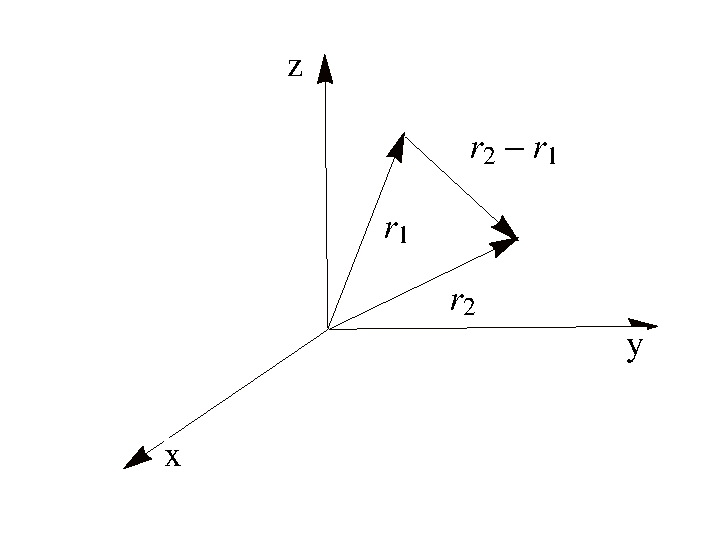
\includegraphics[scale=0.5]{forcacentral}

    \end{minipage}&
    \begin{minipage}{0.45\textwidth}
$$\vec{p_1}=m_1\vec{v_1} \quad \vec{p_2}=m_2 \vec{v_2}$$

$$M=m_1+m_2$$


    \end{minipage}
  \end{tabular}
} 

\frame{\frametitle{Coordenadas reduzidas}

$$\vec{r}=\vec{r_2}-\vec{r_1} \quad \vec{r_G}=\frac{m_1 \vec{r_1} +m_2\vec{r_2}}{M}$$

$$\vec{r_1}=\vec{r_G}+\frac{m_2 \vec{r}}{M} \quad 
\vec{r_2}=\vec{r_G}-\frac{m_1 \vec{r}}{M}$$

$$H=\frac{1}{2}M\dot{\vec{r_G}^2}+\frac{1}{2M}\dot{\vec{r}}^2m_1m_2+V(r)$$ 

$$H=\frac{\vec{p_G}^2}{2M}+\frac{\vec{p}^2}{2\mu}+V(r)$$

$$\mu=\frac{m_1m_2}{m_1+m_2}$$
}

\frame{\frametitle{Hamiltoniano Quântico}
$$\hat{H}=\frac{-\hbar^2}{2M}\nabla^2_G-\frac{\hbar^2}{2\mu}\nabla^2+V(r)$$

$$\Psi(\vec{r_G},\vec{r})=\psi_G(\vec{r_G})\psi(\vec{r})$$

$$\hat{H}\Psi=E_T\Psi$$

$$\left(\frac{-\hbar^2}{2M}\nabla^2_G-\frac{\hbar^2}{2\mu}\nabla^2+V(r)\right)
\psi_G\psi=E_T\psi_G\psi$$

}

\frame{\frametitle{Hamiltoniano Quântico}
$$\psi \frac{-\hbar^2}{2M}\nabla^2_G\psi_G+
\psi_G\left( -\frac{\hbar^2}{2\mu}\nabla^2+V(r)\right)\psi=E_T\psi_G\psi$$

$$\frac{1}{\psi_G} \frac{-\hbar^2}{2M}\nabla^2_G\psi_G+
\frac{1}{\psi}\left( -\frac{\hbar^2}{2\mu}\nabla^2+V(r)\right)\psi=E_T$$

$$E_T=E_G+E$$

}

\frame{\frametitle{Centro de Massa}
$$\frac{-\hbar^2}{2M}\nabla^2_G\psi_G=E_G\psi_G$$

Este é a equação de uma partícula livre em 3D. 
}

\frame{\frametitle{Coordenadas Reduzidas}
$$\left( -\frac{\hbar^2}{2\mu}\nabla^2+V(r)\right)\psi=E\psi$$

}


\frame{\frametitle{Momento Angular Clássico}
Em coordenadas esféricas temos:

$$\vec{L}=m\vec{v}\times \vec{r}$$

$$=m(\dot{\vec{r}}\vec{a_r}+r\dot{\theta}\vec{a_\theta}+r\sin \theta \dot{\phi}\vec{a_\phi})\times \vec{r}$$

$$=m(r^2\dot{\theta}^2\vec{a_\phi}+r^2\sin \theta \dot{\phi}\vec{a_\theta})$$

$$L^2=m^2r^4(\dot{\theta}^2+\sin^2 \theta\dot{\phi ^2})$$

}
\frame{\frametitle{Momento Angular Clássico}

$$\frac{mv^2}{2}=\frac{m}{2}(\dot{r}^2+r^2\dot{\theta}^2+r^2\sin^2 \theta \dot{\phi}^2)$$

$$\frac{mv^2}{2}=\frac{p^2}{2m}=\frac{m}{2}\dot{r}^2+\frac{L^2}{2mr^2}$$

}


\frame{\frametitle{Coordenadas Reduzidas}
$$\left( \frac{p^2}{2m}+V(r)\right)\psi=E\psi$$

$$\left( -\frac{\hbar^2}{2\mu}\nabla^2+V(r)\right)\psi=E\psi$$

$$\nabla^2=\frac{1}{r}\frac{\partial^2}{\partial r^2}r+
\frac{1}{r^2}\left( 
\frac{\partial^2}{\partial \theta^2}+\frac{1}{\tan \theta}\frac{\partial}{\partial \theta}+\frac{1}{\sin^2 \theta} \frac{\partial^2}{\partial\phi^2}
\right)$$

}

\frame{\frametitle{Coordenadas Reduzidas}
$$\hat{L}^2=\left( 
\frac{\partial^2}{\partial \theta^2}+\frac{1}{\tan \theta}\frac{\partial}{\partial \theta}+\frac{1}{\sin^2 \theta} \frac{\partial^2}{\partial\phi^2}
\right)$$

$$\hat{H}=\frac{-\hbar^2}{2\mu}\frac{1}{r}\frac{\partial^2}{\partial r^2}r+
\frac{1}{2\mu r^2}\hat{L}^2+V(r)$$

}

\frame{\frametitle{Coordenadas Reduzidas}
$$\psi (r,\theta, \phi )=R(r)Y_{lm}(\theta,\phi )$$

$$H\psi=\left[ \frac{-\hbar^2}{2\mu}\frac{1}{r}\frac{\partial^2}{\partial r^2}[R(r)r]+V(r)R(r)\right]Y_{lm}(\theta,\phi )+\frac{R(r)}{2\mu r^2}\hat{L}^2Y_{lm}(\theta, \phi)$$

Usando:
$$L^2Y_{lm}=\hbar^2 l(l+1)Y_{lm}$$

$$\left[ \frac{-\hbar^2}{2\mu}\frac{1}{r}\frac{\partial^2}{\partial r^2}[R(r)r]+V(r)R(r)\right]+\frac{\hbar^2l(l+1)}{2\mu r^2}R(r)=ER(r)$$

}

\frame{\frametitle{Dependência Radial}
$$R=R_{kl}(r)$$

$$\left[ \frac{-\hbar^2}{2\mu}\frac{1}{r}\frac{\partial^2}{\partial r^2}[R_{kl}(r)r]+V(r)R_{kl}(r)\right]+\frac{\hbar^2l(l+1)}{2\mu r^2}R_{kl}(r)=E_{kl}R_{kl}(r)$$

}

\section{Átomo de Hidrogênio}

\frame{\frametitle{Átomo de Hidrogênio}

$$V(r)=\frac{-Ze}{4\pi\epsilon_o r}  \quad E<0$$

Substituição de variáveis:

$$\rho =\sqrt{\frac{8\mu|E|}{\hbar^2}}r \quad \beta=\sqrt{\frac{8\mu|E|}{\hbar^2}}$$

$$\lambda=\frac{Ze^2}{4\pi \epsilon_o\hbar}\sqrt{\frac{\mu}{2|E|} }=Z\alpha\sqrt{\frac{\mu c^2}{2|E|} } \quad \alpha=\frac{e^2}{4\pi\epsilon_o\hbar c}$$

$$ \frac{d^2 R}{d\rho^2}+\frac{2}{\rho}\frac{dR}{d\rho}+\left(\frac{\lambda}{\rho}-\frac{1}{4}-\frac{l(l+1)}{\rho^2}\right)R(\rho)=0$$


}

\frame{\frametitle{Substituição de Variáveis}

$$R(\rho)=e^{-\rho /2}\rho^lh(\rho )$$

$$\frac{d^2 h}{d\rho^2}+\left( \frac{2l+2}{\rho} -1 \right)\frac{dh}{d\rho}
+\frac{1}{\rho}(\lambda -l-1)h=0$$

}
\frame{\frametitle{Resolução por Série}

$$h(\rho )=\sum_k a_k\rho^k$$

Substituindo na equação:

$$\sum_k^\infty a_k\left[ k(k-2)\rho^{k-2} +k\left( \frac{2l+2}{\rho} -1\right)\rho^{k-1}
+(\lambda-l-1)\rho^{k-1} \right] =0$$

Manipulando essa equação temos que:

$$a_{k+1}=\frac{k+l+1-\lambda}{(k+1)(k+2+2l)}a_k$$
}

\frame{\frametitle{Comportamento Assintótico}

$$a_{k+1}\sim \frac{1}{k}a_k  \quad a_k\sim \frac{1}{k!}$$

Isso implica que:

$$h(\rho )\sim e^\rho \quad R(\rho )=e^{-\rho /2}\rho^l h(\rho)\sim e^{\rho/2}$$

ou seja $R$ diverge no infinito. O que não é fisicamente aceitável. 
}

\frame{\frametitle{Autovalores}

Para evitar a divergência, escolhemos:

$$a_{k+1}=\frac{k+l+1-\lambda}{(k+1)(k+2+2l)}a_k$$

$$\lambda=n_r+l+1$$

Número quântico principal:

$$n=n_r+l+1$$

$$n_r\geq 0 \quad n\geq l+1$$
}

\frame{\frametitle{Espectro}
$$\lambda=n$$

$$n^2=\frac{Z^2\alpha^2\mu c^2}{2|E|}\quad |E_n|=\frac{\mu c^2Z^2\alpha^2}{2n^2} $$

Mesmo Resultado que o modelo de Bohr!
}

\frame{\frametitle{Autofunções}

$$R(r)e^{-\rho /2}\rho^l h(\rho)$$

Com a escolha de $\lambda$ as funções $h$ passam a ser polinômios,
que na Literatura são conhecidos por polinômios de Laguerre. 

$$h(\rho) =L_{n-l-1}^{2l+1} (\rho )$$

$$L_n^\eta =\sum_{m=0}^n \binom{n+\eta}{n-m}\frac{(-\rho)^m}{m!} $$

}

\frame{\frametitle{Autofunções}
Temos também que:

$$\rho =\frac{2Z}{a_o n}r$$

onde temos:

$$a_o=\frac{\hbar}{\mu c \alpha}$$

Finalmente temos:

$$R_{nl}(r)=e^{\frac{-Zr}{na_o}}\left(\frac{2Zr}{na_o} \right)^lL_{n-l-1}^{2l+1}\left(\frac{2Zr}{na_o}\right)$$
}

\frame{\frametitle{Autofunções}
$$\psi(r.\theta,\phi)=\sum_{nlm}A_{nlm}Y_{lm}(\theta,\phi) e^{\frac{-Zr}{na_o}}\left(\frac{2Zr}{na_o} \right)^lL_{n-l-1}^{2l+1}\left(\frac{2Zr}{na_o}\right)$$
}

\frame{\frametitle{Degenerescência}

$$n=n_r+l+1$$

\begin{description}
\item[$n=1$] $n_r=0 \quad l=0$ deg=1
\item[$n=2$] deg=4
  \begin{itemize}
  \item $n_r=0 \quad l=1$ deg=3
  \item $n_r=1 \quad l=0$ deg=1
  \end{itemize}
\item[$n=2$] deg=9
\end{description}
}


\frame{\frametitle{Degenerescência}
Caso geral:

$$\sum_{l=0}^{l_{max}} (2l+1)=\sum_{l=0}^{n-1}(2l+1)=n^2$$
}


\frame{\frametitle{Degenerescência}
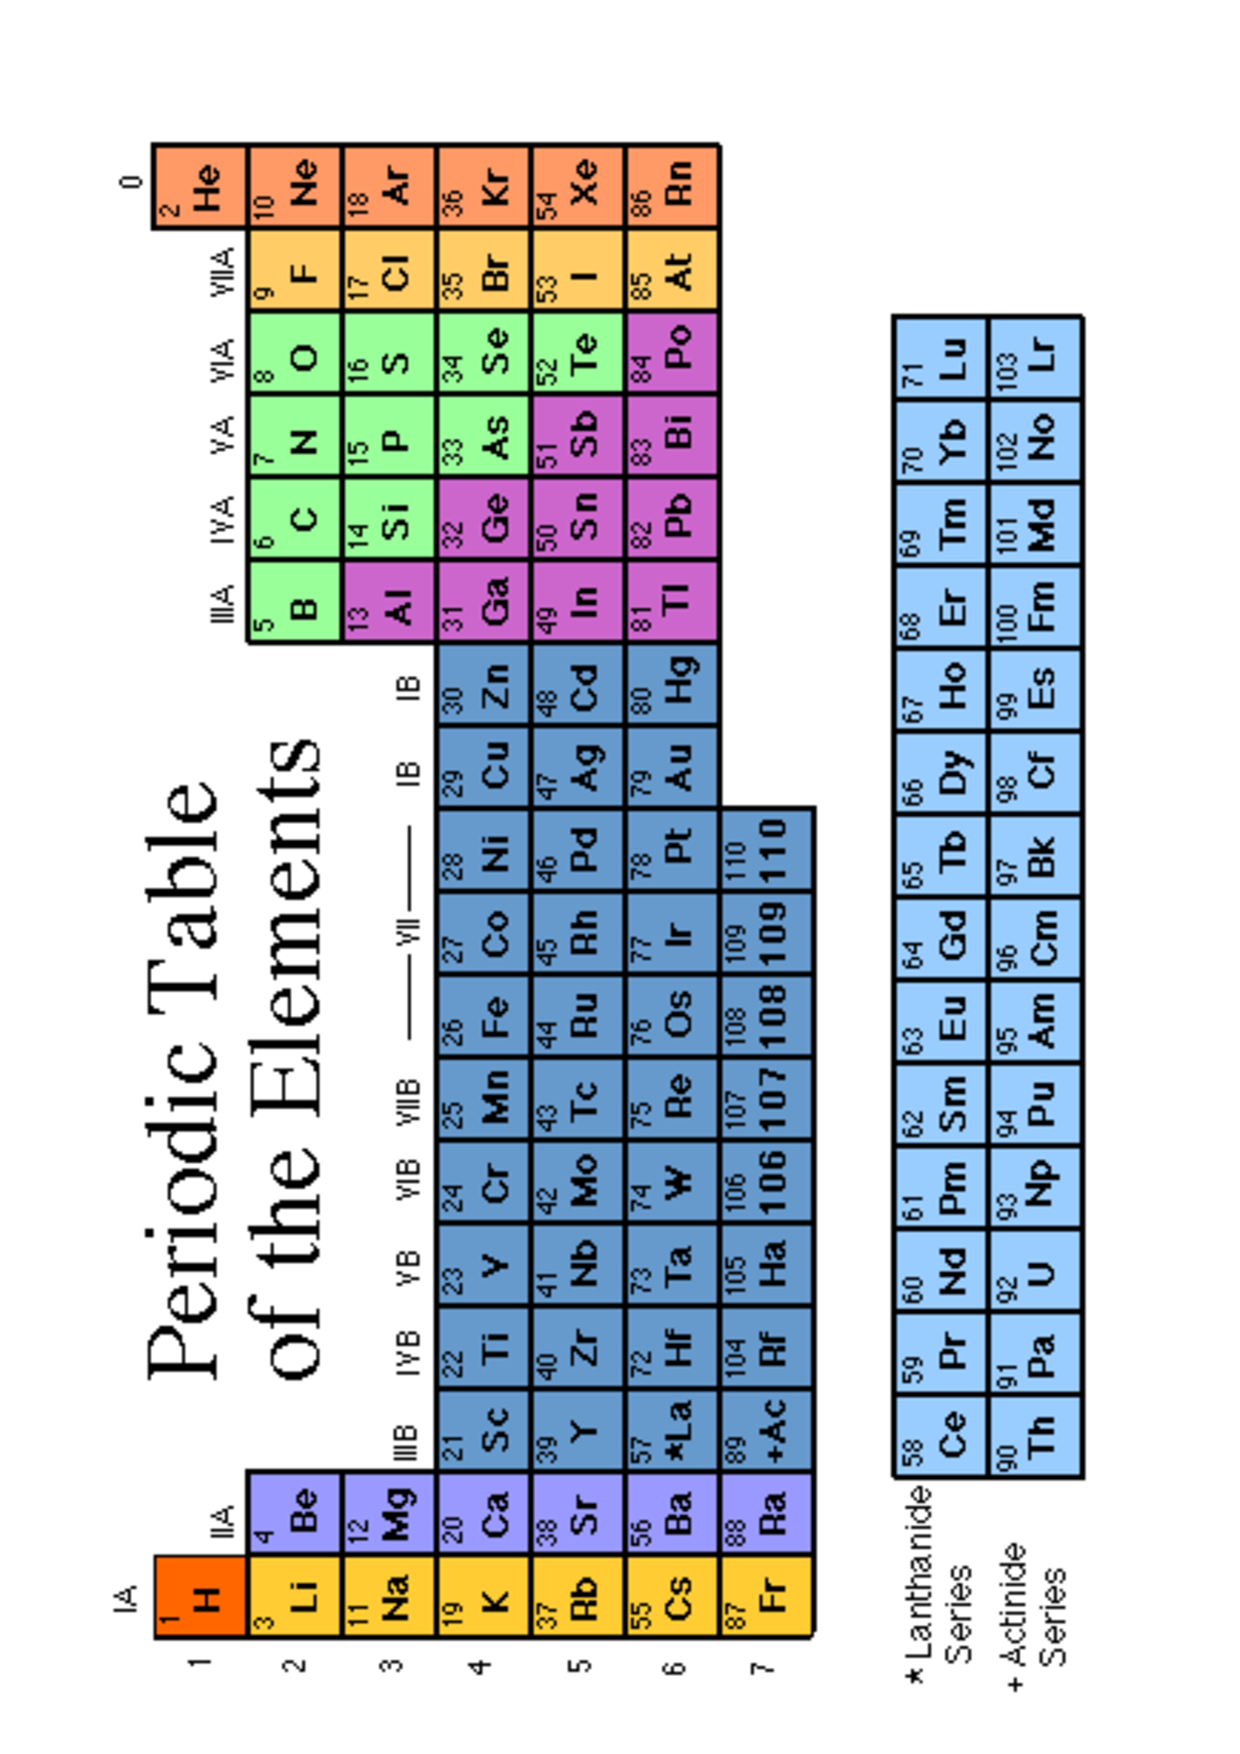
\includegraphics[scale=0.3, angle=270]{periodic1.pdf}
}
\frame{\frametitle{Radial Distribution }
  \begin{center}
    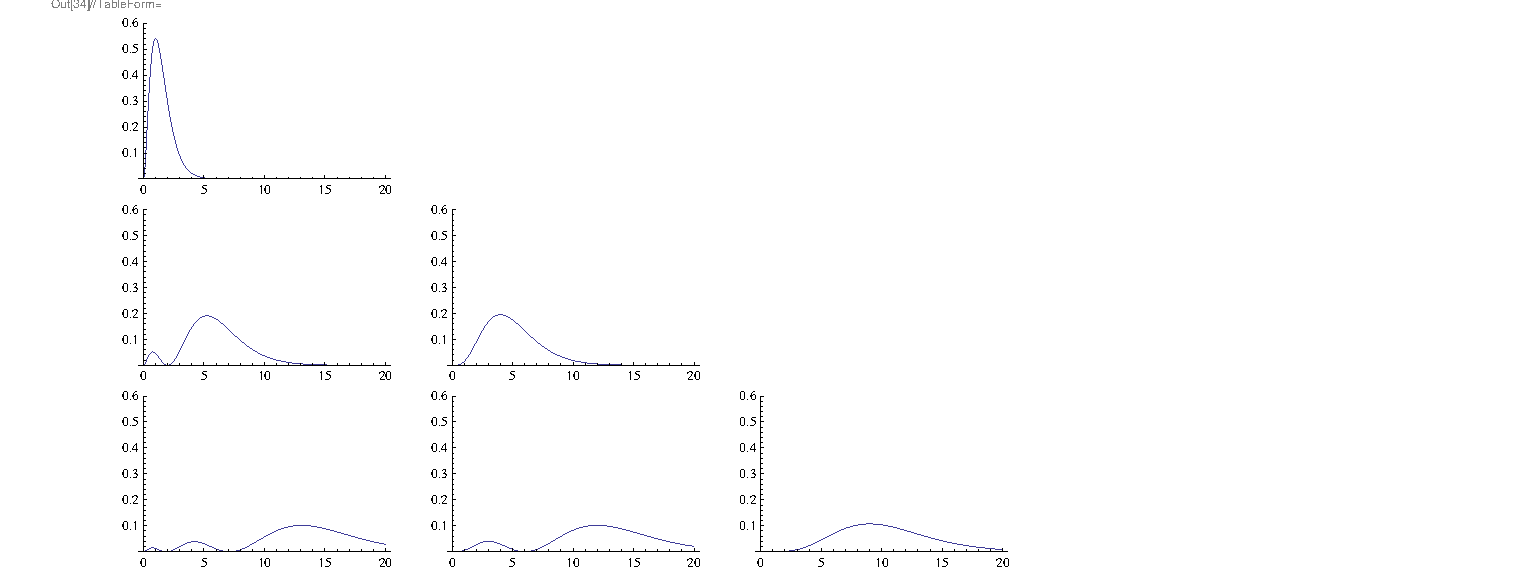
\includegraphics[scale=0.5]{radialdis}
  \end{center}
}

\frame{\frametitle{Radial Distribution $n=2$ $ l=1$ $m=1$}

  \begin{center}
    \includegraphics[scale=0.5]{radialdis3d}
  \end{center}
}

\end{document}
